\scanpage{21}
\figure{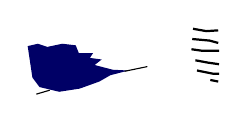
\begin{tikzpicture}[x=1cm,y=1cm]
\fill[blue!40!black] (0,.33)--(.13,.36)--(.25,.32)--(.44,.36)--(.61,.34)--(.65,.24)--(.83,.24)--(.79,.18)--(.94,.16)--(.85,.09)--(1.08,.03)--(1.28,.02)--(1.05,-.04)--(.91,-.12)--(.66,-.21)--(.4,-.25)--(.15,-.19)--(.06,-.07)--cycle;
\draw[thin] (1.23,.01)--(1.52,.07) (.11,-.28)--(.28,-.23);
\draw[thick] (2.1,.55)--(2.27,.52)--(2.42,.53) (2.09,.42)--(2.31,.4)--(2.42,.37) (2.08,.29)--(2.22,.27)--(2.43,.27) (2.13,.15)--(2.29,.12)--(2.43,.1) (2.15,.02)--(2.35,-.02)--(2.43,-.02) (2.32,-.1)--(2.42,-.12);
\end{tikzpicture}}

\rotatebox{180}{\begin{minipage}{.65\linewidth}
\uline{Def} \quad $\mathbf F$ sheaf on $X$ is

\deleted{$X$}
\end{minipage}}
\margin{20}

